\documentclass[aspectratio=169,11pt]{beamer}
\usetheme{Boadilla}
\usepackage[T1]{fontenc}
\usepackage[polish]{babel}
\usepackage{lmodern}
\usepackage{amsmath}
\usepackage{graphicx}

\title{Czy wahadło może mierzyć czas?}
\subtitle{Model małych wychyleń i dane przykładowe}
\author{Opracowanie przykładowe}
\date{27 października 2026}

\begin{document}

\begin{frame}
  \titlepage
\end{frame}

\begin{frame}{Pytanie}
  Czy dłuższe wahadło wykonuje jeden cykl wolniej?
  \begin{itemize}
    \item Okres $T$ mierzymy w sekundach.
    \item Długość $L$ mierzymy w metrach.
    \item Porównamy model z pięcioma danymi syntetycznymi.
  \end{itemize}
\end{frame}

\begin{frame}{Model małych wychyleń}
  \begin{block}{Okres wahadła matematycznego}
   $$
      T=2\pi\sqrt{\frac{L}{g}},\qquad g=9{,}81\,\mathrm{m/s^2}.
   $$
  \end{block}
  Zależność od $L$ jest pierwiastkowa. Podwojenie długości
  zwiększa okres $\sqrt{2}$ razy.
\end{frame}

\begin{frame}{Dane przykładowe}
  \centering
  \begin{tabular}{c|ccccc}
    $L$ (m) & $0{,}20$ & $0{,}40$ & $0{,}60$ & $0{,}80$ & $1{,}00$ \\
    \hline
    $T$ (s) & $0{,}90$ & $1{,}27$ & $1{,}55$ & $1{,}80$ & $2{,}01$
  \end{tabular}
  \vspace{0.6cm}

  To liczby przygotowane do ćwiczenia, nie zapis pomiaru laboratoryjnego.
\end{frame}

\begin{frame}{Dane i model}
  \centering
  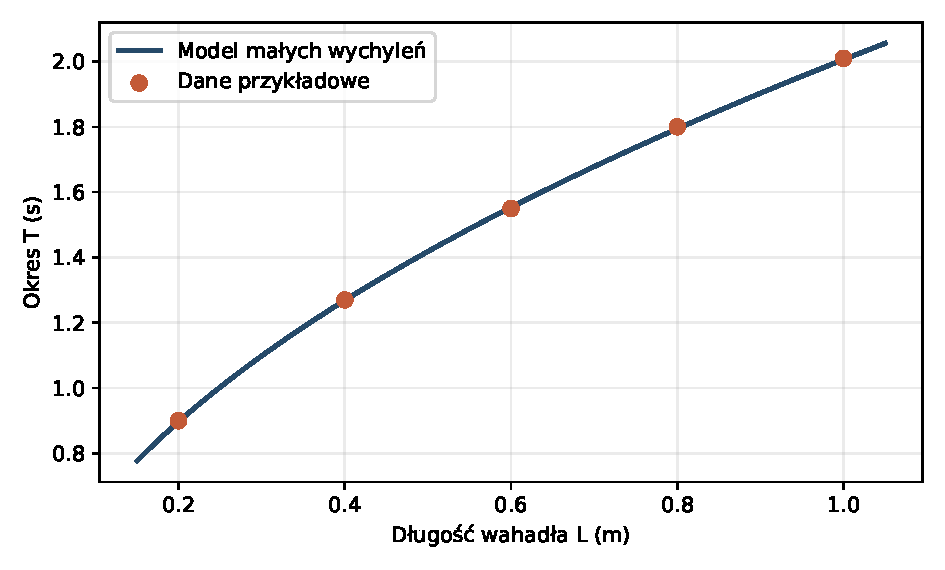
\includegraphics[width=0.76\linewidth]{../raport/wykres.pdf}

  \small Punkty: dane syntetyczne. Linia: model małych wychyleń.
\end{frame}

\begin{frame}{Porównanie liczb}
  \begin{columns}[T]
    \begin{column}{0.47\textwidth}
      \begin{block}{Dla $L=1{,}00\,\mathrm{m}$}
        Model: około $2{,}0061\,\mathrm{s}$.

        Tabela: $2{,}01\,\mathrm{s}$.
      \end{block}
    \end{column}
    \begin{column}{0.47\textwidth}
      \begin{block}{Największa różnica}
        $|T_{\mathrm{tabela}}-T_{\mathrm{model}}|<0{,}006\,\mathrm{s}$
        dla pięciu punktów.
      \end{block}
    \end{column}
  \end{columns}
\end{frame}

\begin{frame}{Ograniczenia}
  \begin{enumerate}
    \item Wzór zakłada małe wychylenia i pomijalny opór.
    \item Brakuje protokołu pomiaru i niepewności.
    \item Zgodność liczb nie jest weryfikacją eksperymentalną.
  \end{enumerate}
\end{frame}

\begin{frame}{Wniosek}
  W przygotowanych danych okres rośnie z długością zgodnie z trendem
  modelu. Do oceny rzeczywistego doświadczenia potrzebne byłyby
  pomiary, powtórzenia i oszacowanie niepewności.
\end{frame}

\begin{frame}{Źródła i pliki}
  \begin{itemize}
    \item \href{https://openstax.org/books/university-physics-volume-1/pages/15-4-pendulums}{OpenStax, \emph{University Physics}, sekcja 15.4}: model wahadła.
    \item \href{https://matplotlib.org/stable/}{Matplotlib}: wykres wygenerowany ze skryptu.
    \item Dane, kod i bibliografia: folder \texttt{../raport/} w repozytorium.
  \end{itemize}
\end{frame}

\end{document}
